\chapter{Revenus de placement}
\section{Introduction et objectifs}
\subsection{Introduction}
Ce chapitre traite des dividendes, des intérêts et autres revenus de placement, des gains en capital figurant sur des feuillets de renseignements, des frais financiers et des frais d'intérêts.


\subsection{Objectifs}
\begin{itemize}[label=\twemoji{check mark button}]
	\item Expliquer et déclarer les dividendes provenant de sociétés canadiennes imposables, privées et publiques;
	\item Au fédéral, reconnaître les circonstances où il est avantageux d'inclure les dividendes reçus par le conjoint dans le revenu du contribuable;
	\item Déclarer les intérêts et autres revenus de placement provenant de sources canadiennes et de sources étrangères;
	\item Remplir la Feuille de travail fédérale pour les lignes~12000, 12010 et 12100 pour les dividendes imposables de sociétés canadiennes, les intérêts et autres revenus de placement et inclure les totaux sur les déclarations de revenus T1 et TP-1;
	\item Remplir la Feuille de travail fédéral pour la ligne~22100 pour les frais financiers et les frais d'intérêts et inclure les totaux sur les déclarations de revenus T1 et TP-1;
	\item Expliquer ce qu'il y a faire avec les gains en capital ou pertes en capital figurant sur des feuillets de renseignements;
	\item Expliquer l'exigence de déclaration de la vente d'une résidence principale;
	\item Expliquer ce qu'on entend par règles d'attribution et comment les appliquer;
	\item Réclamer les frais engagés pour gagner des revenus de placement;
	\item Au Québec, calculer le rajustement des frais de placement et compléter l'annexe correspondante;
	\item Expliquer pourquoi les contribuables peuvent devoir verser des cotisations au Fonds des services de santé du Québec.
\end{itemize}


\subsection{Sujets du chapitre}
\begin{itemize}
	\item Introduction à la feuille de travail fédérale
	\item Régles d'attribution
	\item Frais financiers
	\item Dividende
	\item Gain en capital
	\item Intérêt
	\item Vente de résidence principal
\end{itemize}



\section{Revenus de placement}
\begin{intro}
	Tous les revenus de placements au Canada et en provenance du reste du monde, qu'ils soient déclarés ou non sur des feuillets de renseignements, doivent être déclarés dans les déclarations de revenus fédérales et du Québec.
\end{intro}
Les revenus de placement sont divisés en quatre catégories:
\begin{itemize}
	\item Dividendes
	\item Intérêts
	\item Les gains en capital
	\item Autres revenus de placement
\end{itemize}

Les montants déclarés sont les mêmes sur les deux déclarations. Cependant, il existe de petites différences dans la manière dont les revenus sont déclarés dans chaque déclaration, selon la source et le type de revenus de placement reçus.



\section{Feuille de travail fédérale}
Au fédéral, les dividendes, les intérêts et les autres revenus de placement doivent être détaillés sur la \href{https://www.canada.ca/fr/agence-revenu/services/formulaires-publications/trousses-impot-toutes-annees-imposition/trousse-generale-impot-prestations/5000-d1.html}{Feuille de travail fédérale}. Les gains en capital sont déclarés séparément sur l'annexe 3.

Au Québec, il n'y a pas de formulaire équivalent. Une note explicative doit accompagner les revenus de placement qui n'ont pas été déclarés sur les feuillets de renseignements. La feuille de travail fédérale peut être jointe à la TP-1. Les gains en capital sont déclarés séparément sur l'annexe G. 



\section{Revenus de dividendes}
\begin{intro}
	Si vous détenez des actions dans une société, qu'elle soit publique ou privée, vous vous attendez (espérez) être récompensé en tant qu'actionnaire. Cette récompense peut prendre la forme d'une part des bénéfices annuels et/ou d'une augmentation de la valeur de vos actions. 
	
	Sur cette page, nous nous concentrerons sur la façon dont les bénéfices réalisés par la société et distribués aux actionnaires sont traités aux fins de l'impôt.
\end{intro}

\index{Dividende}
Lorsqu'une société distribue une part de son bénéfice après impôt à ses actionnaires, cette distribution est appelée un \textbf{dividende}. Ils peuvent être versés en argent ou en actions. 

Avant de distribuer des dividendes à ses actionnaires, la société a dû payer des impôts sur ses bénéfices. En d'autres termes, les dividendes sont payés à partir des bénéfices après impôts. 

Au Canada, le gouvernement applique un traitement fiscal particulier à un actionnaire qui reçoit des dividendes de sociétés canadiennes imposables privées ou publiques. 

Ce traitement ne s'applique pas aux dividendes reçus de sociétés étrangères. 


\subsection{Dividendes}
Plusieurs termes vont circuler en ce qui concerne les dividendes, les voici:
\begin{itemize}[label=\twemoji{check box with check}]
	\item Dividende déterminé d'une société publique;
	\item Dividende déterminé d'une société privée;
	\item Dividende autre qu'un déterminé d'une société publique;
	\item Dividende autre qu'un déterminé d'une société privée;
	\item Dividende ordinaire d'une société publique;
	\item Dividende ordinaire d'une société privée;
	\item Dividende réel;
	\item Dividende majoré;
	\item Dividende étranger.
\end{itemize}

L'utilisation de chacun des termes est indiquée dans la table~\ref{table:dividendes}.
\begin{table}
	\centering
	\begin{tabular}{|l|c|}
		\hline
		\rowcolor{LightGreen}\multicolumn{2}{|c|}{\textbf{Dividendes}}                                                         \\ \hline
		\textbf{Description}                                      &                      \textbf{Termes}                       \\ \hline
		Dividende déterminé d'une société publique                &                     Utilisé au Fédéral                     \\
		Dividende déterminé d'une société privée                  &                        et au Québec                        \\ \hline
		Dividende autre qu'un déterminé d'une société publique *  &                     Utilisé seulement                      \\
		Dividende autre qu'un déterminé d'une société privée *    &                         au Fédéral                         \\ \hdashline
		Dividende ordinaire d'une société publique *              &                     Utilisé seulement                      \\
		Dividende ordinaire d'une société privée *                &                         au Québec                          \\ \hline
		Dividende réel **                                         &                     Utilisé au Fédéral                     \\
		                                                          &                        et au Québec                        \\ \hline
		Dividende majoré ***                                      &                     Utilisé au Fédéral                     \\
		                                                          &                        et au Québec                        \\ \hline
		Dividende étranger                                        &                     Utilisé au Fédéral                     \\
		                                                          &                        et au Québec                        \\ \hline\hline
		\multicolumn{2}{|l|}{* Le dividende autre que déterminé a la même signification que le dividende}                      \\
		\multicolumn{2}{|l|}{ordinaire. Les dividendes sont tout simplement \og appelés \fg{} différemment selon}              \\
		\multicolumn{2}{|l|}{le gouvernement.}                                                                                 \\
		\multicolumn{2}{|l|}{** Ce terme indique le montant qui a bien été reçu par le contribuable. Ce }                      \\
		\multicolumn{2}{|l|}{montant n'a pas subi de majoration encore.}                                                       \\
		\multicolumn{2}{|l|}{*** Ce terme indique que le dividende a subi une majoration selon le taux en }                    \\
		\multicolumn{2}{|l|}{vigueur basé sur le genre de société.}                                                            \\
		\multicolumn{2}{|l|}{\textbf{Remarque}. Il existe un autre terme, celui de \og dividende non déterminé \fg{}. Il est } \\
		\multicolumn{2}{|l|}{rarement utilisé dans la documentation. La définition est la même que le}                         \\
		\multicolumn{2}{|l|}{dividende ordinaire (autre que déterminé).}                                                       \\ \hline
	\end{tabular}
	\caption{Dividendes}
	\label{table:dividendes}
\end{table}


\subsubsection{Dividendes déterminés et dividendes ordinaires (autres que les dividendes déterminés)}
Quelle est la différence entre un dividende déterminé et un dividende ordinaire (autre que déterminé)?
\begin{enumerate}
	\item Le dividende déterminé provient généralement d'une société imposée au taux général d'imposition des sociétés, tandis que
	\item Le dividende non déterminé provient généralement d'une entreprise qui se qualifie de société privée sous contrôle canadien (SPCC), qui bénéficie d'un taux d'impôt inférieur à l'impôt général des sociétés pour sa première tranche de \numprint{500000}~\$ de revenus actifs.
\end{enumerate}


\subsubsection{Sociétés publiques ou privées}
Quelle est la différence entre une société publique et une société privée?  La réponse est courte, mais vous donnera une petite idée afin que vous puissiez faire la différence.
\begin{enumerate}
	\item Une société canadienne privée n'a pas d'actions cotées en bourse;
	\item Une société canadienne publique a des actions cotées en bourse.
\end{enumerate}

\subsubsection{Dividendes imposables et majoration}
Lorsqu'un contribuable reçoit un dividende d'une société canadienne imposable, le montant qu'il doit inclure dans son revenu est le dividende reçu plus une \og majoration \fg{}. Le dividende versé par la société est appelé \og dividende réel \fg{}.

Le dividende majoré est appelé \og dividende imposable \fg{}. Dû au fait que les sociétés publiques et privées ne sont pas imposées au même taux, il y a deux majorations, en fonction de la société qui verse le dividende. Voir table~\ref{table:MajorationDividende}.
\begin{table}
	\centering
	\begin{tabular}{|c|c|c|c|c|}
		\hline
		 Types de  &  Taux de   & Société  &  \multicolumn{2}{c|}{Taux du crédit d'impôt appliqué sur le}  \\
		Dividendes & majoration &          &             \multicolumn{2}{c|}{dividende majoré}             \\ \cline{4-5}
		           &            &          &  Fédéral   &                      Québec                      \\ \hline
		Déterminé  &   38 \%    & Publique & 15,0198 \% &                    11,70 \% *                    \\ \hline
		Ordinaire  &   15 \%    &  Privée  & 9,0301 \%  &                    3,42 \% **                    \\ \hline\hline
		\multicolumn{5}{|l|}{Dans le guide TP-1, on montre une méthode de calcul basée sur les dividendes} \\
		\multicolumn{5}{|l|}{réels:}                                                                       \\
		\multicolumn{5}{|l|}{* 16,1460 \% en utilisant les dividendes réels}                               \\
		\multicolumn{5}{|l|}{** 3,9330 \% en utilisant les dividendes réels}                               \\ \hline
	\end{tabular}
	\caption{Majoration et taux du crédit sur le dividende majoré}
	\label{table:MajorationDividende}
\end{table}


\subsection{Crédit d'impôt pour dividendes}
Afin de tenir compte de l'impôt payé (au taux réduit ou général) par la société canadienne qui paie le dividende, la loi accorde un crédit d'impôt non remboursable au contribuable qui reçoit le dividende. C'est ce qu'on appelle un crédit d'impôt pour dividendes. 

Bien que le Québec utilise les mêmes taux de majoration que le gouvernement fédéral, les pourcentages utilisés par le Québec pour calculer le crédit d'impôt pour dividende sont différents. Il y a donc deux montants différents pour le crédit d'impôt qui peuvent être réclamés, selon le type de dividende versé par une société.

La majoration et le \acrfull{cid} sont calculés et déclarés sur les feuillets de renseignements que les sociétés canadiennes doivent remettre à leurs actionnaires lorsqu'elles versent des dividendes de 50~\$ ou plus au cours de l'année. 

Les taux de majoration et du crédit d'impôt peuvent être assujettis à un ajustement s'il y a une réduction du taux d'imposition général sur le revenu des sociétés.

Voir table~\ref{table:MajorationDividende}.

\begin{note}
	Le traitement fiscal est appliqué seulement aux dividendes canadiens et non aux dividendes étrangers.
\end{note}

\subsubsection{Feuillets de renseignements et relevés}
La majoration et les crédits d'impôt pour dividendes sont calculés et indiqués sur les feuillets de renseignements que les sociétés canadiennes doivent émettre aux actionnaires lorsqu'elles leur versent des dividendes de 50~\$ ou plus durant l'année. 

Cependant, le contribuable qui ne reçoit pas de feuillets doit quand même déclarer le montant imposable du dividende reçu en faisant lui-même le calcul.

Les tableaux de la feuille de travail fédérale fournissent maintenant la méthode pour effectuer ce calcul.

Les feuillets de renseignements qui servent à indiquer les dividendes versés sont les: 
\begin{itemize}
	\item T3/RL-16;
	\item T4PS/RL-25;
	\item T5/RL-3;
	\item T5013/RL-15. 
\end{itemize}

Tables~\ref{table:MajorationDividende} et \ref{table:Releves}.
\begin{table}
	\centering
	\begin{tabular}{|c|c|c|c|c|c|}
		\hline
		\textbf{Document} &     \textbf{Description}      &          \multicolumn{4}{c|}{\textbf{Case du dividende}}           \\ \cline{3-6}
		                  &                               & \textbf{Code} & \textbf{Réel} & \textbf{Majoré} & \textbf{Crédit}  \\
		                  &                               &               &               &                 & \textbf{d'impôt} \\ \hline
		       T3         &  État des revenus de fiducie  &       D       &      49       &       50        &        51        \\ \cline{3-6}
		                  &                               &       O       &      23       &       32        &        39        \\ \hline
		      T4PS        & État des attributions et des  &       D       &      30       &       31        &        32        \\
		                  & paiements dans le cadre d'un  &               &               &                 &                  \\ \cline{3-6}
		                  &  régime de participation des  &       O       &      24       &       25        &        26        \\
		                  &    employés aux bénéfices     &               &               &                 &                  \\ \hline
		       T5         & État des revenus de placement &       D       &      24       &       25        &        26        \\ \cline{3-6}
		                  &                               &       O       &      10       &       11        &        12        \\ \hline
		      T5013       &    État des revenus d'une     &       D       &      132      &       133       &       134        \\ \cline{3-6}
		                  &     société de personnes      &       O       &      129      &       130       &       131        \\ \hline\hline
		\multicolumn{6}{|c|}{D: Dividende Déterminé \qquad O: Dividende Ordinaire}                                             \\ \hline
	\end{tabular}
	\caption{Feuillets d'impôt fédéral}
	\label{table:Feuillets}
\end{table}

\begin{table}
	\centering
	\begin{tabular}{|c|c|c|c|c|c|}
		\hline
		\textbf{Document} &  \textbf{Description}  &          \multicolumn{4}{c|}{\textbf{Case du dividende}}           \\ \cline{3-6}
		                  &                        & \textbf{Code} & \textbf{Réel} & \textbf{Majoré} & \textbf{Crédit}  \\
		                  &                        &               &               &                 & \textbf{d'impôt} \\ \hline
		      RL-3        &  Revenus de placement  &       D       &      A1       &        B        &        C         \\ \cline{3-4}
		                  &                        &       O       &      A2       &                 &                  \\ \hline
		      RL-15       & Montants attribués aux &       D       &      6A       &       6-1       &        44        \\ \cline{3-4}
		                  & membres d'une société  &       O       &      6B       &                 &                  \\
		                  &      de personnes      &               &               &                 &                  \\ \hline
		      RL-16       &   Revenus de fiducie   &       D       &      C1       &        I        &        J         \\ \cline{3-4}
		                  &                        &       O       &      C2       &                 &                  \\ \hline
		      RL-25       & Revenus provenant d'un &       D       &      A1       &        F        &        G         \\ \cline{3-4}
		                  & régime d'intéressement &       O       &      A2       &                 &                  \\ \hline\hline
		\multicolumn{6}{|c|}{D: Dividende Déterminé \qquad O: Dividende Ordinaire}                                      \\ \hline
	\end{tabular}
	\caption{Relevés d'impôt du Québec}
	\label{table:Releves}
\end{table}


\subsection{Traitement fiscal}
Dans une situation où il n'y a aucun feuillet de renseignements, on doit examiner le relevé ou l'état de compte que la société (payeur) a émis au contribuable, ou toute autre information qu'il a pu recevoir à ce sujet. On doit déterminer s'il s'agit d'une société privée ou d'une société publique (cotée à la bourse). 

\subsubsection{Feuille de travail fédérale}
Le montant des dividendes imposables doit être inscrit sur la \href{https://www.canada.ca/fr/agence-revenu/services/formulaires-publications/trousses-impot-toutes-annees-imposition/trousse-generale-impot-prestations/5000-d1.html}{feuille de travail fédérale} à la section \og \textbf{lignes~12000 et 12010 – Montant imposable des dividendes de sociétés canadiennes imposables} \fg{}.

\subsection{Comment inscrire des dividendes sur la TP-1}
Il n'y a pas d'équivalent à la feuille de travail fédérale pour le TP-1, cependant le montant total des dividendes imposables de la ligne~12000 sur la T1 doit être inscrit à la ligne~128 de la TP-1.

À titre informatif, les contribuables sont tenus d'inscrire le montant réel des dividendes déterminés à la ligne~166 et le montant réel des dividendes ordinaires à la ligne~167 de la TP-1.


\subsection{Dividendes étrangers}
Les dividendes reçus d'une société étrangère doivent être inscrits en dollars canadiens à la section \og \textbf{ligne~12100 - Intérêts et autres revenus de placement} \fg{} de la feuille de calcul fédérale.

Au fédéral et au Québec, les dividendes étrangers ne sont pas assujettis au traitement fiscal. Autrement dit, ces dividendes ne sont pas assujettis à une majoration et ils ne sont pas admissibles au crédit d'impôt pour dividendes. Inscrivez le montant total en dollars canadiens à la ligne~12100 de la T1 et à la ligne~130 de la TP-1.

\subsection{Crédit d'impôt pour dividendes}
Les contribuables qui déclarent des dividendes ordinaires et déterminés de sociétés canadiennes imposables peuvent réclamer un crédit d'impôt pour dividendes aux lignes~40425 de la T1 et 415 de la déclaration TP-1. 

\begin{note}
	Depuis le 1\ier{} janvier 2020, au Québec, pour bénéficier de la totalité du crédit d'impôt pour dividendes ordinaires ou déterminés, le particulier doit être résident du Québec au 31 décembre de l'année d'imposition.
\end{note}


\subsection{Dividendes d'un régime de participation des employés aux bénéfices}
Un \acrfull{rpeb} est un régime pour lequel les cotisations de l'employeur sont établies en fonction des bénéfices réalisés par l'entreprise. Les versements sont faits à une fiducie créée au nom des employés. Le fiduciaire du RPEB ne verse réellement les revenus que la fiducie génère que lorsque les employés quittent le régime. Il leur attribue plutôt, tous les ans, les revenus générés sous forme d'intérêts, de dividendes ou de gains en capital. Les dividendes ainsi attribués sont indiqués sur un T4PS et un relevé 25. Ils sont traités de la même façon que les autres dividendes.


\subsection{Dividendes attribués par une fiducie}
Des dividendes peuvent être payés à une fiducie aussi bien qu'à des particuliers. Par la suite, les montants attribués sont reportés sur un T3 et un relevé 16. Ils doivent être traités comme les autres dividendes. Il y a des fiducies testamentaires et des fiducies non testamentaires. Une fiducie créée suite au décès d'une personne, appelée \og Succession de\dots{} \fg{}, est un exemple d'une fiducie testamentaire.


\subsection{Dividendes sur gains en capital}
Les dividendes sur gains en capital sont des revenus qui proviennent d'une société de placements, d'une société de fonds communs de placement ou d'une société de placements hypothécaires. Ils sont indiqués sur un T5 et un relevé 3. Ils doivent être reportés comme des gains en capital, sans être majorés. Aucun crédit d'impôt pour dividendes ne peut être réclamé pour ce type de revenus. Sujet discuté plus loin dans ce chapitre.

Les dividendes sur gains en capital payés par les sociétés résidant aux États-Unis ne sont pas considérés, aux fins des impôts fédéral et provincial, comme des dividendes ni comme des gains en capital. Reporter les dividendes à la section  \og ligne~12100 - Intérêts, autres revenus de placements \fg{} comme revenus de source étrangère de la feuille de travail fédérale.


\subsection{Choix de déclarer les dividendes du conjoint}
Au fédéral, un contribuable peut choisir d'inclure dans son revenu, tous les dividendes imposables de sociétés canadiennes imposables qui ont été reçus par son époux(se) ou conjoint(e) de fait.

Cela ne peut être fait \textbf{que si}, en excluant les dividendes du revenu de leur conjoint  et par conséquent réduisant le revenu net du conjoint, il permet au contribuable de réclamer ou d'augmenter le montant pour époux ou conjoint de fait.

Le contribuable doit également réclamer le crédit d'impôt pour dividendes associé dans sa déclaration de revenus.

En transférant les dividendes imposables, le contribuable augmente son propre revenu imposable.

Par conséquent, ce transfert ne devrait être effectué que si l'augmentation de l'impôt dû au transfert est inférieure au crédit d'impôt provenant du montant pour époux ou conjoint de fait majoré plus le crédit d'impôt pour dividendes transféré.

Au Québec, une telle initiative est inutile, car le crédit d'impôt pour dividendes qui n'est pas utilisé sera transféré au conjoint via la ligne~431.

\rqg[s]{24 et 62}



\section{Exercice 1}
\setcounter{question}{0}
\begin{question}
	François a reçu, de la société Bell Canada, un chèque de 100~\$ pour un dividende qui lui a été versé. Toutefois, il n'a reçu aucun feuillet de renseignements. Bell Canada est une société publique canadienne imposable.
\end{question}
\setcounter{sousQuestion}{0}
\begin{sousQuestion}
	Quel est le montant imposable du dividende reçu? Montrez votre calcul.
\end{sousQuestion}
Le montant des dividendes imposables est de 138~\$, calculé 100~\$ $\times$ 1,38.

\begin{sousQuestion}
	Quels sont les crédits d'impôt pour dividendes qu'il peut demander sur la T1 et la TP-1? Montrez vos calculs.
\end{sousQuestion}
Le montant du crédit d'impôt fédéral pour dividendes est de 20,73~\$ sur la T1.
\[ 138~\$ \times 15,0198~\% = 20,73~\$ \]

Le montant du crédit d'impôt du Québec pour dividendes est de 16,15~\$.
\[ 138~\$ \times 11,70~\% = 100~\$ \times 16,1460~\% =  16,15~\$ \]
\begin{question}
	Nicole Gingras a reçu les feuillets de renseignements cf. figures~\ref{fig:chap6Exercice1T3} et \ref{fig:chap6Exercice1RL16}. De plus, le 15~septembre~2023, elle a reçu un chèque de 32~\$ pour un dividende de la société Corona, pour lequel elle n'a eu aucun feuillet. Corona est une société privée canadienne imposable.
	
	Complétez la section appropriée de la \href{https://www.canada.ca/fr/agence-revenu/services/formulaires-publications/trousses-impot-toutes-annees-imposition/trousse-generale-impot-prestations/5000-d1.html}{Feuille de travail fédérale}, et reportez le résultat aux lignes appropriées de sa T1 et sa TP-1.
	\begin{figure}
		\centering
		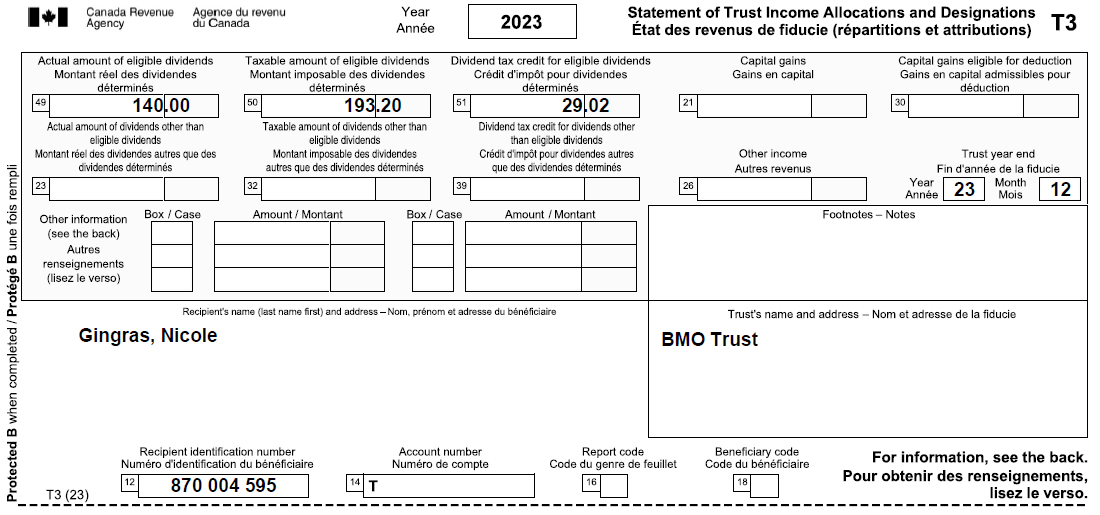
\includegraphics[width=.9\textwidth]{exercice/6-1/Q2/T3.png}
		\caption[]{Exercice 1, T3}
		\label{fig:chap6Exercice1T3}
	\end{figure}
	\begin{figure}
		\centering
		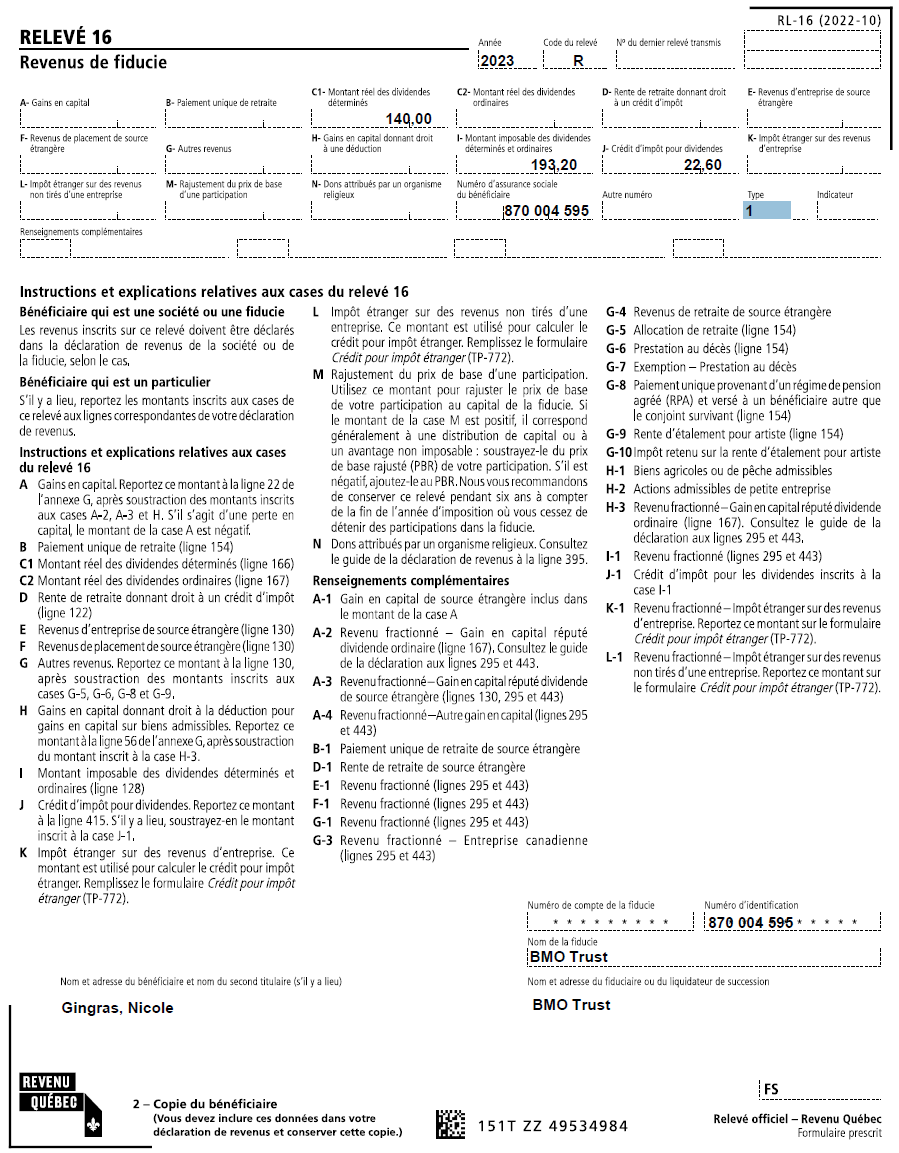
\includegraphics[width=.9\textwidth]{exercice/6-1/Q2/RL16.png}
		\caption[]{Exercice 1, RL-16}
		\label{fig:chap6Exercice1RL16}
	\end{figure}
\end{question}
T1, ligne~12000 = 230~\$ (193,20~\$ + 36,80~\$)

T1, ligne~12010 = 36,80 ( 32~\$ x 1,15 )

TP-1, ligne~128 = 230~\$

TP-1, ligne~166 = 140~\$

TP-1, ligne~167 = 32~\$

Feuille de travail fédérale: figure~\ref{fig:chap6Exercice1FeuilleTravail}

\begin{figure}
	\centering
	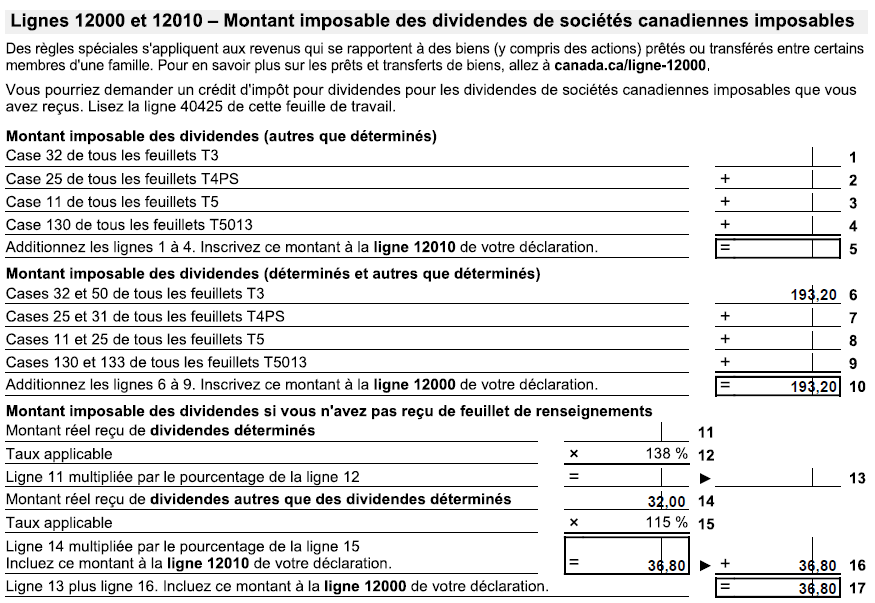
\includegraphics[width=.9\textwidth]{exercice/6-1/Q2/FeuilleTravail.png}
	\caption[]{Exercice 1, Feuille de travail fédérale}
	\label{fig:chap6Exercice1FeuilleTravail}
\end{figure}

\begin{question}
	Denis, un contribuable résident du Québec, a reçu d'une société américaine, un dividende de 500~USD.
\end{question}

\setcounter{sousQuestion}{0}
\begin{sousQuestion}
	Quel est le montant du dividende imposable aux fins de l'impôt sur le revenu du Canada?
\end{sousQuestion}
500~USD $\times$ 1,3497 = 674,85~CAD (1,3497 est le taux de conversion moyen CAD-USD en 2023).

Les 500~USD doivent être convertis en dollars canadiens. Comme aucune date n'est fournie, on utilise le taux de change annuel moyen.

Notez qu'aucune majoration ne doit être effectuée sur les dividendes provenant d'une source étrangère.

\begin{sousQuestion}
	Dans quelle section de la feuille de travail fédérale doit-on déclarer ce montant?
\end{sousQuestion}
Dans la section \og \textbf{ligne~12100 – Intérêts et autres revenus de placements} \fg{} à la ligne~6 de la feuille de travail fédérale.

\begin{question}
	Au fédéral, dans quelle situation un contribuable peut-il choisir d'inclure dans son revenu, les dividendes que son/sa époux(se) ou conjoint(e)de fait a reçus durant l'année?
\end{question}
Cela ne peut se faire que si le transfert des dividendes augmente ou crée le montant pour époux ou conjoint de fait que le contribuable peut demander. Ceci est réalisé en réduisant le revenu net de l'époux(se) ou du conjoint(e) de fait par la suppression du revenu de dividendes imposable.



\section{Revenus d'intérêts}
\begin{intro}
	Les intérêts sont le rendement, la contrepartie ou l'indemnité reçue pour l'utilisation ou la détention d'une somme d'argent appartenant à une autre personne. Ils sont souvent exprimés en pourcentage annuel du capital prêté ou déposé, et calculés sur une base quotidienne, mensuelle, trimestrielle ou annuelle.
\end{intro}
Les intérêts sont reportés aux lignes~12100 de la T1 et 130 de la TP-1.


\subsection{Intérêts provenant des institutions financières}
Les intérêts d'un compte bancaire, d'un compte à une caisse populaire ou à toute autre institution financière, sont payés au contribuable à mesure qu'ils sont gagnés. Ces institutions financières doivent émettre des T5 et relevé 3 pour les intérêts gagnés de 50~\$ ou plus. Les intérêts de source canadienne sont indiqués aux cases~13 du T5 et D du relevé~3. 

Même si aucun feuillet de renseignements n'est émis, comme pour les montants inférieurs à 50~\$, le contribuable doit tout de même déclarer tous les intérêts reçus


\subsubsection{Comptes communs}
Si un contribuable et son conjoint (époux ou conjoint de fait) ont un compte bancaire en commun, les intérêts gagnés sur ce compte ne sont pas automatiquement partagés à parts égales 50/50. Cela dépend de qui a versé les sommes déposées dans le compte et des montants déposés.


\subsection{Contrats de placement à long terme (acquis après 1989)}
L'expression \og contrat de placement \fg{} signifie ordinairement tous les genres de placement sur lesquels le contribuable connaît d'avance les bénéfices qu'il pourra en retirer. Il peut s'agir des dépôts à terme, des obligations d'épargne du Québec et des certificats de placement garantis. Pour la majorité des contrats de placement à long terme, les intérêts sont payés à l'échéance ou lors de l'encaissement de l'investissement, et non annuellement.

Le contribuable qui a investi dans des contrats à long terme acquis après 1989 doit quand même déclarer annuellement les intérêts accumulés sur ces investissements, que ces intérêts lui soient versés ou non au cours de l'année d'imposition. 

Il faut déclarer les intérêts accumulés jusqu'à la date anniversaire du contrat, et non pas les intérêts accumulés durant l'année civile. Par exemple, la date anniversaire d'un contrat acheté le 1er juillet 2022 est le 30~juin~2023, et les intérêts accumulés jusqu'à cette date doivent être reportés sur les déclarations de 2023. Ils sont inscrits sur des T5 et relevés 3.


\subsection{Titres de créance}
Les \og titres de créance \fg{} comprennent des obligations, débentures, effets, billets, hypothèques, bons du Trésor ou d'autres titres semblables. Les institutions financières sont tenues de déclarer les dispositions et rachats des titres de créance. À cet effet, les contribuables reçoivent des feuillets~T5008, État des opérations sur titres, et relevé 18, Transactions de titres.


\subsection{Bons du Trésor à long terme et obligations à coupons détachés}
Les bons du Trésor à long terme ou une obligation à coupons détachés sont des titres émis par le gouvernement du Canada ou celui d'une province pour une courte période, soit 3, 6 ou 12 mois. Les bons du Trésor sont vendus à escompte, c'est-à-dire que les investisseurs paient moins que sa valeur nominale. La différence entre la valeur nominale du bon du Trésor et le prix que le contribuable a payé constitue l'escompte.

Si le contribuable conserve son titre jusqu'à l'échéance, il encaisse la valeur nominale et la différence entre le produit de disposition (c'est-à-dire le montant encaissé à l'échéance) et le coût du titre (c'est-à-dire le prix payé au moment de l'achat) doit être déclarée comme un revenu d'intérêts. Ces intérêts doivent être reportés à la section ligne~12100 – Intérêts et autres revenus de placements de la feuille de travail fédérale.

Le produit de disposition d'un bon du Trésor est inscrit à la case~21 du feuillet~T5008. Au Québec, il est inscrit à la case~21 intitulée \og Produit de l'aliénation ou paiement \fg{} du relevé 18. Le coût du titre pourrait être inscrit aux cases~20 des feuillets~T5008 et relevé 18. S'il ne l'est pas, l'information doit être obtenue d'une autre façon (par exemple à partir du relevé ou état de compte que le contribuable a reçu au moment de l'acquisition du titre en question).


\subsubsection{T5008 et relevé 18}
Le feuillet~T5008 et le relevé 18 n'indiquent pas le montant qui doit être inclus dans le revenu du contribuable. Ce montant doit être calculé manuellement comme suit: 
\begin{itemize}
	\item le produit de disposition \textbf{moins} le coût du titre.
\end{itemize}

\begin{note}
	Ces deux feuillets de renseignements sont également utilisés pour reporter d'autres transactions de titres. Dans la plupart des cas, la disposition indiquée sur ces feuillets est traitée comme une disposition de biens en capital (étudiée un peu plus loin dans ce chapitre).
\end{note}


\subsection{Obligations d'épargne du Canada}
\subsubsection{Fait historique}
Il n'a pas été possible d'acheter des \acrfull{oec} depuis novembre 2017. La dernière série d'obligations d'épargne du Canada est arrivée à échéance en 2021. Voici une ventilation des différents types d'obligations qui pouvaient être achetées auparavant. 

\subsubsection{Obligations à intérêt régulier}
Les obligations à intérêt régulier versent un intérêt simple une fois par an à la date anniversaire de l'achat jusqu'à l'échéance. Le dépôt direct des intérêts était obligatoire et les intérêts devaient être déclarés annuellement.

\subsubsection{Obligations à intérêt composé}
Les personnes qui détenaient des obligations à intérêts composés ne reçoivent aucun intérêt tant que l'obligation n'a pas été encaissée. Entre-temps, la partie des intérêts était réinvestie chaque année afin que les intérêts que gagne le détenteur d'obligations soient composés. Les intérêts gagnés sur les obligations à intérêts composés devaient être déclarés annuellement.

\subsubsection{Obligations d'épargne du Canada -- Obligations à prime du Canada}
Les Obligations d'épargne du Canada traditionnelles n'étaient offertes que par le biais du programme d'épargne-salaire qui permettait aux employés des entreprises participantes d'acheter les obligations au moyen de retenues sur la paie.


\subsection{Obligations d'épargne du Québec}
Les \acrfull{oeq} sont émises par Épargne Placements Québec.

\subsubsection{Obligations à intérêts simples}
Les contribuables peuvent toujours acheter des obligations d'épargne du Québec.

Les intérêts courus sur les OEQ à intérêts simples sont payés tous les ans.

Les intérêts gagnés doivent être déclarés tous les ans.

\arcg[s]{13 et 14}

\rqg{24}



\section{Autres revenus de placement}
\begin{intro}
	Certains revenus de placement doivent être déclarés à la section \og ligne~12100 - Intérêts et autres revenus de placement \fg{}, puis reportés à la ligne~12100 de la T1 et à la ligne~130 de la TP-1.
\end{intro}


\subsection{Revenu de placement canadien}
Certains revenus de placement qui proviennent d'institutions canadiennes doivent être déclarés à la section ligne~12100 – Intérêts et autres revenus de placements de la feuille de travail fédérale. Ils sont ensuite reportés aux lignes~12100 de la T1 et 130 de la TP-1. Ces revenus comprennent, entre autres:
\begin{description}
	\item[Remboursements d'impôt] L'avis de cotisation ou de nouvelle cotisation reçu par un contribuable au cours de l'année d'imposition du gouvernement fédéral ou du gouvernement du Québec peut indiquer le montant des intérêts inclus dans le remboursement. L'intérêt en question doit être déclaré dans l'année où il est reçu.
	\item[Revenu de fiducie ou de succession] Les intérêts payés par une fiducie ou une succession constituent un revenu imposable. Il est inscrit à la case~26 du T3 et à la case~G du Relevé 16.
	\item[Société de personnes] Les intérêts d'une société de personnes canadienne sont inscrits à la case~128 du T5013 et à la case~7 du Relevé 15.
	\item[Gains sur polices d'assurance-vie] Lorsqu'une compagnie d'assurance vend une police d'assurance-vie à un contribuable, les revenus accumulés dans son contrat d'assurance peuvent ou non être exonérés d'impôt. Si la police n'est pas exonérée d'impôt, le contribuable recevra un T5 et un Relevé 3 qui l'indiquent à la case~19 du T5 et à la case~J du Relevé 3.
\end{description}

Au fédéral, le montant indiqué à la case~19 du T5 doit être déclaré à la section \og ligne~12100 - Intérêts et autres revenus \fg{} de la feuille de travail fédérale.

Si le contribuable a moins de 65 ans, le montant est alors déclaré à la ligne~12100 de la T1. 

Si le contribuable a 65 ans ou plus, ou s'il a reçu le montant d'assurance-vie suite au décès de son/sa conjoint(e), le montant doit être déclaré à la ligne~11500 de la T1. 

Au Québec, le montant de la case~J du Relevé 3 est reporté à la ligne~122 du TP-1, peu importe les circonstances.
\begin{description}
	\item[Redevances de sources canadiennes] Les redevances qu'un contribuable a reçues pour l'utilisation d'un bien, comme un brevet, un droit d'auteur ou une marque de commerce, sont inscrites à la case~17 du T5 et à la case~H du Relevé 3. Au fédéral, le montant de la case~17 du T5 est inscrit sur la feuille de travail fédérale dans la section \og ligne~12100 - Intérêts et autres revenus de placement \fg{}. Ensuite, le montant est inscrit à la ligne~12100 de la T1.
	
	Toutefois, si le montant comprend des redevances provenant du travail ou de l'invention d'un contribuable, ces redevances doivent être déclarées à la ligne~10400 de la T1.
	
	Au Québec, le montant de la case~H du Relevé 3 est déclaré à la ligne~130 de la déclaration TP-1.
	\item[Autres revenus de placement] Tous les autres revenus de placement de source canadienne sont inscrits à la case~14 du T5 et à la case~E du Relevé 3.
\end{description}


\subsection{Revenus de placement de sources étrangères}
Les intérêts et les autres revenus de placement de sources étrangères doivent être déclarés à la section ligne~12100 – Intérêts et autres revenus de placements de la feuille de travail fédérale. Ils sont ensuite reportés aux lignes~12100 de la T1 et 130 de la TP-1. On y retrouve:
\begin{itemize}
	\item Les revenus de placement étranger, dont les montants versés (bruts) sont inscrits aux cases~15 du T5 et F du relevé 3;
	\item Les revenus étrangers non tirés d'entreprise, cases~25 du T3 et F du relevé 16;
	\item Les dividendes reçus d'une société étrangère;
	\item Tout autre intérêt ou revenu de placement de sources étrangères.
\end{itemize}

Le revenu étranger doit être déclaré en devise canadienne. Le contribuable qui reçoit des revenus en devise étrangère doit les convertir en utilisant le taux de change au moment de la transaction. S'il reçoit des paiements périodiques, il peut utiliser le taux de change moyen pour l'année. Pour les taux de change quotidiens et mensuels, consultez le site Web de la Banque du Canada.

\href{https://www.banqueducanada.ca/taux/taux-de-change/}{Banque du Canada -- Taux de change}



\section{Exercice 2}
\setcounter{question}{0}
\begin{question}
	Jane, conjointe de fait, s'occupe des finances de la famille. Jane a ouvert un compte conjoint au nom du couple. Jane y dépose régulièrement les chèques de paie de son conjoint.
	
	Jane vous remet le T5 et le relevé 3 indiquant les intérêts versés dans le compte.
	
	Dans quelle déclaration de revenus, les intérêts doivent-ils être inscrits? Expliquez votre réponse.
\end{question}
Les intérêts devront être inscrits dans la déclaration de son conjoint, car la source de revenu d'intérêts provient du dépôt des revenus d'emploi de son conjoint.

\begin{question}
	Jean et Lise ont un compte conjoint, dans lequel Jean a versé \numprint{3000}~\$ et Lise, \numprint{1000}~\$. Le T5 et le relevé 3, qu'ils ont reçus, indiquent des intérêts de 400~\$.
	
	Quel montant doit-on inscrire sur chacune de leur déclaration?
\end{question}
Pour Jean, ce sera 300~\$, calculé ainsi:  (\numprint{3000}~\$ / \numprint{4000}~\$)  $\times$  400~\$.

Pour Lise, ce sera 100~\$, calculé ainsi:  (\numprint{1000}~\$ / \numprint{4000}~\$)  $\times$  400~\$.

\begin{question}
	Vincent a reçu un T5008 et un relevé 18  indiquant \numprint{100000}~\$ comme produit de disposition d'un bon du Trésor. Le prix d'achat du bon du Trésor, selon le relevé de courtage, a été de \numprint{98573}~\$.
	
	Comment ces montants doivent-ils être traités dans la déclaration de Vincent? 
\end{question}
Il doit déclarer la différence entre les deux montants, soit \numprint{1427}~\$, comme un revenu d'intérêt à la ligne~12100 de la T1 et à la ligne~130 de la TP-1.

\begin{question}
	Nommer trois types de placement à long terme.
\end{question}
\begin{enumerate}
	\item Dépôt à terme;
	\item Obligations d'épargne du Québec;
	\item Certificat de placement garanti.
\end{enumerate}

\begin{question}
	Quand les intérêts doivent-ils être déclarés pour les contrats de placement à long terme émis après 1989?
\end{question}
Les intérêts doivent être déclarés à tous les ans, qu'ils aient été versés ou non.

\begin{question}
	Pour quel type d'obligation d'épargne du Canada et d'obligation d'épargne du Québec l'intérêt est-il payé chaque année?
\end{question}
Uniquement pour les obligations à intérêt régulier ("R") émises par le Québec. Il n'y a plus d'intérêt payable sur les Obligations d'épargne du Canada.

\begin{question}
	Thomas a reçu 50~\$ de redevances d'une société canadienne. Le montant est inscrit aux cases~17 du T5 et H du relevé 3.
	
	À quelles lignes de ses T1 et TP-1 doit-il reporter ce montant? Expliquez votre réponse.
\end{question}
Au fédéral, si le montant inscrit à la case~17 du T5 comprend des redevances sur un ouvrage ou sur une invention dont Thomas est l'auteur, ce dernier doit l'inscrire à la ligne~10400 de sa T1. Autrement, il doit le déclarer à la section ligne~12100 – Intérêts et autres revenus de placements et ensuite le reporter à la ligne~12100 de sa T1.

Au Québec, il doit inscrire le montant de la case~H du relevé 3 à la ligne~130 de sa TP1.

\begin{question}
	Fabienne Dorion a reçu le T3 de la figure~\ref{fig:chap6Exercice2T3} et RL-16 de la figure~\ref{fig:chap6Exercice2RL16}.
	
	\begin{figure}
		\centering
		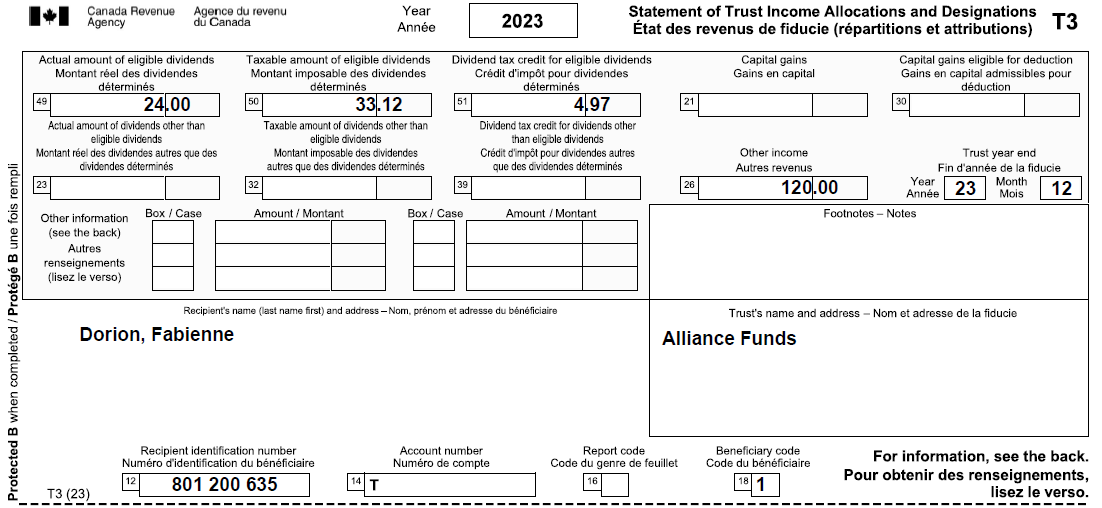
\includegraphics[width=.9\textwidth]{exercice/6-2/Q8/T3.png}
		\caption[]{Exercice 2, T3}
		\label{fig:chap6Exercice2T3}
	\end{figure}
	
	\begin{figure}
		\centering
		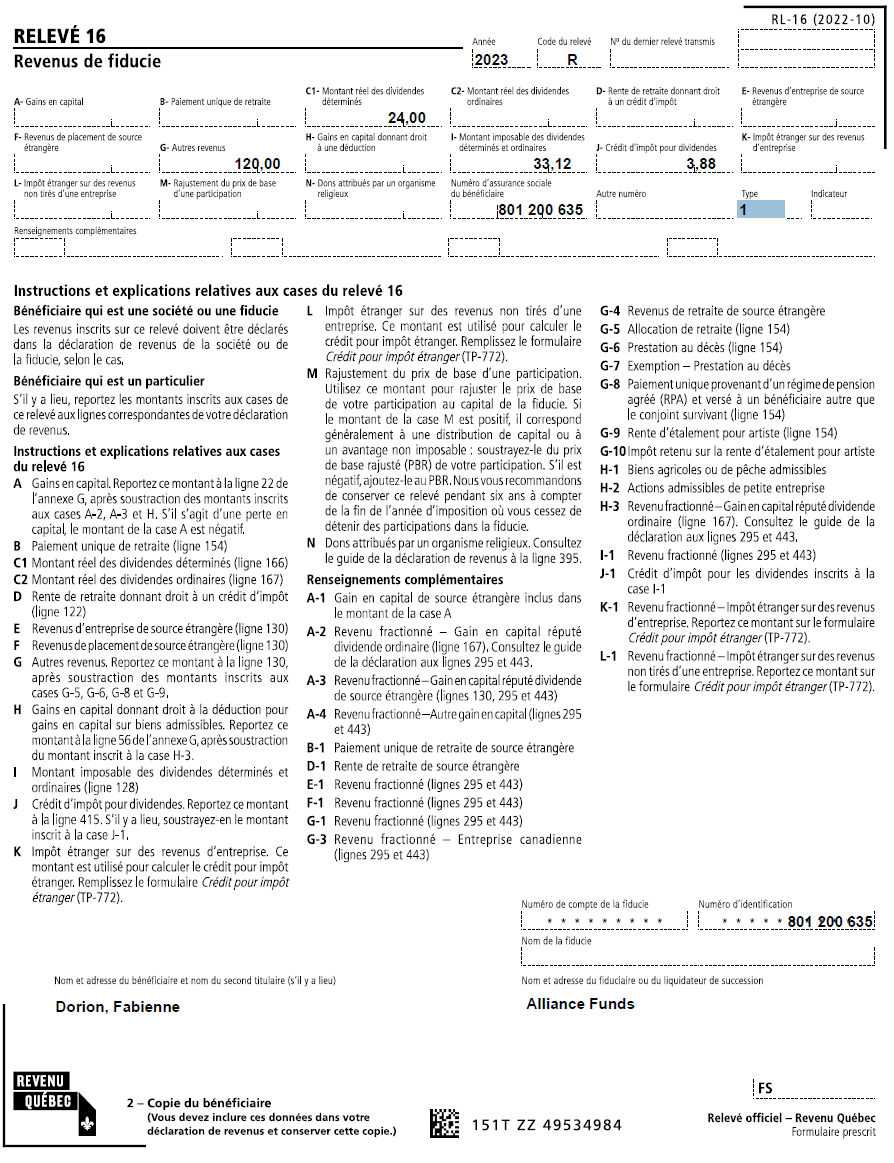
\includegraphics[width=.9\textwidth]{exercice/6-2/Q8/RL16.png}
		\caption[]{Exercice 2, RL-16}
		\label{fig:chap6Exercice2RL16}
	\end{figure}
\end{question}

\setcounter{sousQuestion}{0}
\begin{sousQuestion}
	À quelle ligne de la T1 et de la TP-1 Fabienne doit-elle déclarer le montant de la case~26 du T3 et de la case~G du RL-16?
\end{sousQuestion}
Les 120~\$ de la case~26 du T3 doivent être déclarés à la ligne~13000 de la T1. Les 120~\$ de la case~G du relevé 16 doivent être déclarés à la ligne~130 de la TP1.

\begin{sousQuestion}
	À quelle ligne de la T1 et de la TP-1 Fabienne doit-elle déclarer le montant à la case~51 du T3 et à la case~J du RL-16? 
\end{sousQuestion}
Le crédit d'impôt pour dividendes de 4,97~\$ du T3 est inscrit à la ligne~40425 de la T1.

Le crédit d'impôt pour dividendes de 3,88~\$ du RL-16 est inscrit à la ligne~415 de la TP1.



\section{Gains en capital}
\begin{intro}
	Un gain en capital (ou une perte en capital) est une expression utilisée en fiscalité pour parler d'un profit réalisé (ou d'une perte subie) lors de la vente d'un bien, autre qu'un bien détenu uniquement dans le but de le revendre.
\end{intro}

En fait, on parle ici d'un bien en capital ou d'une \og immobilisation \fg{}. On dit également qu'un bien qui a une valeur durable est un bien en capital. En voici des exemples:
\begin{itemize}
	\item Les valeurs, comme les actions et les obligations;
	\item Les biens locatifs, comme les bâtiments et les terrains;
	\item Les biens d'entreprise, tels les bâtiments, les terrains et les fournitures; 
	\item Les biens à usage personnel (chalets, bateaux, peintures et antiquités);
\end{itemize}

Les cryptomonnaies ne sont pas considérées comme ayant cours légal par l'ARC et Revenu Québec, mais plutôt comme un actif numérique. Les transactions utilisant des cryptomonnaies sont soit considérées comme des revenus d'entreprise, soit comme des transactions d'immobilisations, entraînant un gain ou une perte.

Chaque fois qu'un contribuable dispose d'une immobilisation, il doit déterminer s'il a réalisé un gain en capital ou subi une perte en capital. 

Un gain en capital peut être réalisé lorsque le produit de disposition d'une immobilisation excède son coût total plus toutes les dépenses reliées à la disposition. 

Une perte en capital se produit lorsque l'immobilisation ou l'action est vendu pour une somme inférieure à son coût incluant les dépenses reliées à sa disposition.

La plupart des dispositions de biens en capital ne sont pas reportées sur aucun feuillet de renseignements. Le contribuable doit obtenir lui-même les informations nécessaires, parmi ses documents reliés à l'acquisition et à la disposition du bien, afin de pouvoir effectuer le calcul du gain ou de la perte en capital. 


\subsection{Gain en capital sur le T5008 et relevé 18}
Tel que mentionné plus tôt, la disposition de biens en capital peut être reportée sur le feuillet~T5008 et le relevé 18. Toutefois, les informations fournies sur ces feuillets sont rarement suffisantes pour calculer le gain ou la perte en capital du contribuable. Les informations manquantes comprennent autres entre:
\begin{itemize}
	\item Les frais reliés à l'acquisition du titre;
	\item Les frais reliés à la disposition du titre;
	\item S'il y a lieu, tout ajustement au coût de base du titre après son acquisition;
	\item Le détail de toutes les acquisitions et dispositions de biens qui sont identiques et détenus par le contribuable.
\end{itemize}

\begin{note}
	Ce cours traite uniquement des gains en capital qui sont indiqués sur des feuillets, tels que les T5, T3, T4PS, ainsi que les relevés 3, 16 et 25.
\end{note}


\subsection{Dividende sur gain en capital}
les dividendes sur les gains en capital de source canadienne doivent être déclarés comme gains en capital. Ils sont déclarés sur un T5/Relevé 3 comme indiqué dans la  table~\ref{table:DividendeGainCapital}.
\begin{table}
	\centering
	\begin{tabular}{|c|c|}
		\hline
		Feuillet fiscal & Case \\ \hline
		      T5        &  18  \\ \hline
		   Relevé 3     &  I   \\ \hline
	\end{tabular}
	\caption{Dividende sur gain en capital}
	\label{table:DividendeGainCapital}
\end{table}


\subsection{Fonds communs de placement}
La majorité des gains en capital réalisées sur les opérations des fonds communs de placement sont indiquées sur des feuillets de renseignements.

Un fonds commun de placement est établi sous forme de fiducie et permet aux investisseurs individuels disposant de temps, capital et expertise limités de mettre en commun leurs ressources pour acquérir des parts dans un portefeuille diversifié géré par des professionnels de l'investissement.

Il y a des gains en capital sur les opérations réalisées par l'intermédiaire de fonds communs de placement. En effet, les gestionnaires de fonds achètent et vendent régulièrement des titres détenus dans le fonds, et chacune des transactions peut entraîner un gain ou une perte en capital, selon que les titres sont vendus à un prix supérieur ou inférieur à leur coût.

Puiqu'un fonds commun de placement est une fiducie, les gains en capital conservent leur identité lorsqu'ils sont distribués aux investisseurs individuels. Ainsi, les gains en capital réalisés par la fiducie et attribués aux investisseurs sur un T3/Relevé 16 et T4PS/Relevé 25 comme  dans la  table~\ref{table:GainsCapitalFCP}.
\begin{table}
	\centering
	\begin{tabular}{|c|c|}
		\hline
		Feuillet fiscal & Case \\ \hline
		      T5        &  21  \\ \hline
		   Relevé 16    &  A   \\ \hline
		     T4PS       &  34  \\ \hline
		   Relevé 25    &  B   \\ \hline
	\end{tabular}
	\caption{Gains en capital fonds communs de placement}
	\label{table:GainsCapitalFCP}
\end{table} 

\subsubsection{Vente de fonds communs de placement}
Si un contribuable vend des parts d'un fonds commun de placement, la différence entre le prix d'achat des parts et leur prix de vente constitue également un gain ou une perte en capital. Le gain réalisé ou la perte subie n'est pas déclaré sur les feuillets de renseignements. Le coût et le produit apparaîtraient sur les rapports de transaction émis par le courtier. Les gains ou pertes en capital doivent être déclarés aux annexes 3 et G.

Les gains et pertes en capital sur les biens non mentionnés sur les feuillets de renseignements fédéraux ou les relevés du Québec ne seront pas abordés dans ce cours


\subsection{Traitement fiscal}
On utilise les annexes \href{https://www.canada.ca/fr/agence-revenu/services/formulaires-publications/trousses-impot-toutes-annees-imposition/trousse-generale-impot-prestations/5000-s3.html}{3} (fédéral) et \href{https://www.revenuquebec.ca/documents/fr/formulaires/tp/2023-12/TP-1.D.G%282023-12%29.pdf}{G} (Québec) pour calculer les gains en capital imposables. Les gains en capital reçoivent un traitement fiscal spécial. En effet, seulement 50~\% des gains réalisés sont imposables. Ainsi, le total des gains reportés sur les annexes 3 et G est multiplié par 50~\% pour déterminer les gains en capital imposables. Les gains imposables sont reportés aux lignes~12700 de la T1 et 139 de la TP-1.

\begin{note}
	Les dividendes sur gains en capital doivent être reportés aux lignes~17400 de l'annexe 3 et 22 de l'annexe G.
	
	Les gains en capital gagnés par les fonds communs de placement et attribués aux investisseurs doivent être reportés à la ligne~17600 de l'annexe 3 et à la ligne~22 de l'annexe G.
\end{note}

Si le total de tous les gains en capital de l'année et de toutes les pertes en capital de l'année entraîne une perte en capital globale, celle-ci n'est inscrite sur aucune ligne des déclarations de revenus, c'est-à-dire qu'elle ne peut pas être utilisée directement pour réduire le revenu imposable de l'année d'imposition en cours.

Cependant, le contribuable peut reporter la perte en capital pour compenser les gains en capital des années futures ou reporter la perte en arrière pour l'une des trois années d'imposition précédentes.

Ce sujet n'est pas abordé dans ce cours, mais vous pouvez explorer ce sujet en lisant le guide \cat\href{https://www.canada.ca/content/dam/cra-arc/formspubs/pub/t4037/t4037-22f.pdf}{T4037 -- Gains en capital}.



\section{Exigences en matière de déclaration de résidence principale}
\begin{intro}
	Lorsqu'un particulier vend sa maison (ou en dispose autrement) et qu'elle est désignée comme sa résidence principale pour chaque année de propriété, il n'y a pas d'impôt à payer sur tout gain en capital découlant de la vente en raison de l'exemption pour résidence principale.
\end{intro}

La disposition d'une résidence principale doit être déclarée à la page 2 de l'annexe 3, le formulaire \href{https://www.canada.ca/fr/agence-revenu/services/formulaires-publications/formulaires/t2091ind.html}{T2091(IND) – Désignation d'un bien comme résidence principale par un particulier (autre qu'une fiducie personnelle)} et le formulaire \href{https://www.revenuquebec.ca/fr/services-en-ligne/formulaires-et-publications/details-courant/tp-274/}{TP-274 – Désignation d'un bien comme résidence principale} doit être rempli.

Au Fédéral:
\begin{itemize}
	\item 100~\$ pour chaque mois complet depuis la date d'échéance de production initiale jusqu'à la date à laquelle il a soumis sa demande à la satisfaction de l'ARC, jusqu'à un maximum de \numprint{8000}~\$.
\end{itemize}

Au Québec:
\begin{itemize}
	\item 100~\$ pour chaque mois complet depuis la date d'échéance de production initiale, la demande doit avoir été soumise à l'ARC. RQ suivra l'application de l'ARC à ce sujet. La pénalité peut aller jusqu'à un maximum de \numprint{5000}~\$.
\end{itemize}

De plus, si une copie des documents concernant le choix de changement d'utilisation qui a été envoyée à l'ARC n'est pas envoyée au Québec avant la date limite, vous êtes passible d'une pénalité de 25~\$ par jour, jusqu'à concurrence de \numprint{2500}~\$.

Si une maison est détenue conjointement, les deux copropriétaires doivent compléter les détails de la désignation dans leur déclaration de revenus en déclarant la disposition de leur part de la maison.

Lorsque vous faites la désignation de résidence principale à l'annexe 3, vous avez le choix entre trois cases.
\begin{itemize}
	\item La case~1 est utilisée pour désigner la propriété comme résidence principale pour toutes les années de possession - la vente sera entièrement exonérée de taxe.
	\item Si la case~2 ou la case~3 est sélectionnée, la vente n'est que partiellement exonérée. Les règles et les calculs liés à une exemption partielle dépassent le cadre de ce cours. Voir l'illustration ci-dessous pour un exemple de vente d'une résidence principale.
\end{itemize}

\begin{note}
	Le nombre d'années de détention peut être différent du nombre d'années pendant lesquelles la propriété peut être désignée comme résidence principale.
	
	Ce serait le cas lorsqu'un contribuable dispose d'une résidence principale et acquiert une nouvelle résidence principale au cours de la même année.
	
	Pour vous assurer que le contribuable reçoit la totalité de l'exemption pour résidence principale lors de la disposition de la plus récente acquisition de résidence principale: prenez le nombre d'années de possession \textbf{moins UN} pour déterminer le nombre d'années à désigner comme résidence principale (c.-à-d. ligne~1 du formulaire T2091).
	
	De la page 4 du T2091: Un an est accordé par la loi.
	
	La règle ci-dessus ne devrait s'appliquer qu'aux propriétés qui ont été détenues pendant plus d'une année d'imposition. Pour les propriétés qui ont été détenues pendant moins d'un an, au moins une année d'imposition doit être désignée lors de la demande d'exemption pour résidence principale (c.-à-d. ne désignez pas d'années \og zéro \fg{} parce que la propriété n'est pas techniquement désignée comme résidence principale). Cela ne s'appliquera qu'aux cas où l'exemption pour résidence principale peut toujours être demandée en raison du fait que la règle sur les reventes précipitées de biens ne s'applique pas (cette règle est abordée dans la section suivante). 
\end{note}



\section{Revente précipitée de propriétés résidentielles}
\begin{intro}
	Au Canada, la règle sur la revente précipitée impose une taxe sur les propriétés résidentielles vendues dans les 12 mois suivant l'achat. L'objectif est de freiner les achats spéculatifs et de s'assurer que les bénéfices des ventes rapides sont entièrement imposés comme des revenus d'entreprise, plutôt que de bénéficier de taux d'imposition favorables sur les gains en capital. Toutefois, certaines exemptions s'appliquent aux événements de la vie.
\end{intro}
À compter du 1\ier{}~janvier~2023, une nouvelle règle considère que le bénéfice résultant de la cession d'un logement détenu depuis moins de 12 mois est considéré comme un revenu d'entreprise (même s'il aurait été qualifié de gain en capital). Étant donné que le bénéfice est traité comme un revenu d'entreprise et non comme une plus-value, l'exonération pour résidence principale ne sera pas disponible même si le contribuable y a droit par ailleurs (c'est-à-dire que si un contribuable vend son nouveau logement en moins d'un an, il n'aura pas droit à l'exonération pour résidence principale, sauf s'il a droit à l'une des exonérations liées à un événement de la vie mentionnées ci-dessous).

Un bien assujetti à cette nouvelle règle déterminative est appelé \og bien retourné \fg{}. Il comprend les biens locatifs ainsi que les biens utilisés à des fins personnelles. Le terme n'inclut pas les biens qui auraient été traités comme des stocks indépendamment de la nouvelle règle.

Cette règle ne s'applique pas si la disposition du bien résulte de l'un des événements suivants de la vie:
\begin{itemize}
	\item Le décès du contribuable ou d'une personne qui lui est liée;
	\item Une personne liée qui rejoint le ménage du contribuable ou le contribuable qui rejoint le ménage d'une personne liée (par exemple, naissance d'un enfant, adoption, soins d'un parent âgé);
	\item La rupture du mariage ou de l'union de fait du contribuable, lorsque celui-ci a vécu séparé de son époux ou conjoint de fait pendant au moins 90 jours avant la disposition;
	\item Une menace pour la sécurité personnelle du contribuable ou d'une personne liée (p. ex., la menace de violence familiale);
	\item Le contribuable ou une personne liée souffre d'un handicap ou d'une maladie grave;
	\item Une cessation involontaire de l'emploi du contribuable ou de son époux ou conjoint de fait;
	\item Une réinstallation admissible du contribuable ou de son époux ou conjoint de fait (c.-à-d. que le contribuable ou son époux a le droit de déduire des frais de déménagement);
	\item L'insolvabilité du contribuable (par exemple, en raison d'une accumulation de dettes);
	\item La destruction ou l'expropriation du bien (p. ex., lorsque le bien est détruit en raison d'une catastrophe naturelle ou d'origine humaine).
\end{itemize}

Lorsqu'un bien est détenu pendant 12 mois ou plus, la question de savoir si les bénéfices de la cession sont imposés en tant que revenus d'entreprise reste une question de fait. Le fait qu'un contribuable détienne un bien immobilier pendant plus d'un an ne signifie pas qu'il sera automatiquement considéré comme une plus-value et qu'il pourra bénéficier de l'exonération pour résidence principale (c'est-à-dire que si un contribuable gagne sa vie en achetant et en revendant plusieurs biens immobiliers, il doit toujours déclarer ces revenus en tant que revenus professionnels, même s'il décide de conserver chacun de ses biens pendant 366 jours).

Chaque fois qu'un logement est vendu (y compris un immeuble locatif), la nouvelle section Revente précipitée de biens à la page 3 de l'annexe 3 doit être remplie. Si le bien a été détenu pendant plus d'un an, le contribuable répondra \og Non \fg{} à la question de la ligne~17905. Si le bien a été détenu pendant moins d'un an, il est nécessaire de répondre \og Oui \fg{}, et si l'un des événements de la vie s'applique, il doit être sélectionné pour la ligne~17906.

Si un bien a été détenu pendant moins d'un an et qu'aucun événement de la vie ne s'applique, une déclaration d'entreprise est requise et l'exemption pour résident principal ne peut pas être demandée pour le bien.

Si Revenu Québec estime qu'une revente de propriété a été précipitée, les bénéfices réalisés sur cette revente seront considérés comme un revenu d'entreprise entièrement imposable et doit être déclaré aux lignes~12 et 22 de l'annexe L.



\section{Règles d'attribution}
\begin{intro}
	Les revenus de placement sont normalement déclarés par le bénéficiaire. Cependant, il existe des exceptions pour les époux ou conjoints de fait et les mineurs.
\end{intro}

Les contribuables des tranches d'imposition élevées se sont vite rendu compte qu'il serait plus avantageux de transférer tout ou partie de leur capital à des membres de la famille à faible revenu pour qu'ils l'investissent afin qu'il soit moins imposé. Sans surprise, le gouvernement a réagi en édictant certaines règles pour prévenir la perte de revenus due à de telles tactiques.

Pour empêcher cette stratégie, la \textbf{Loi de l'impôt sur le revenu} du Canada et la \textbf{Loi sur les impôts du Québec} comprennent une série de règles précises qui limitent la possibilité du contribuable de réduire ses obligations fiscales en fractionnant ses revenus parmi les membres de sa famille. Ces règles sont appelées les \og règles d'attribution \fg{}, car leur but premier est d'attribuer les revenus d'un bien transféré à l'auteur du transfert.


\subsection{Biens qui génèrent des revenus}
Les règles d'attribution s'appliquent aux biens qui génèrent des revenus et qui sont prêtés ou transférés à un époux ou un conjoint de fait ou à une personne de moins de 18 ans qui est liée au contribuable (enfant, petit-enfant, frère, sœur, neveu, nièce).

Les biens qui génèrent des revenus comprennent notamment:
\begin{itemize}[label=\twemoji{check box with check}]
	\item Des actions (pouvant générer des revenus de dividendes);
	\item Des obligations ou autres placements (pouvant générer des intérêts);
	\item Des immeubles de location (pouvant générer des revenus de location);
	\item L'argent (pouvant être donné ou prêté à une personne qui l'utilise pour gagner des revenus de placement)
\end{itemize}.

Les règles d'attribution ne s'appliquent pas au bien transféré aux membres de la famille âgés de 18 ans ou plus (autres que les époux ou conjoints de fait). Toutefois, elles s'appliquent lorsque le bien est prêté à une telle personne.

Des règles spécifiques s'appliquent aux biens transférés à l'époux ou conjoint de fait, ainsi qu'à un enfant mineur. Ils sont étudiés en détail dans ce chapitre.


\subsection{Transfert de bien}
Un transfert de bien peut se faire sous l'une des formes suivantes:
\begin{itemize}
	\item Un don gratuit;
	\item Un prêt sans intérêt;
	\item Un prêt à un taux d'intérêt inférieur au taux prescrit par le gouvernement. Les règles d'attribution ne s'appliquent pas si le prêt porte intérêt au taux prescrit ou à un taux commercial, et que les intérêts accumulés sont versés dans les 30 jours qui suivent la fin de l'année d'imposition;
	\item Une vente à un prix inférieur à sa juste valeur marchande (JVM). Les règles d'attribution ne s'appliquent pas si le bien a été transféré ou vendu à sa juste valeur marchande.
\end{itemize}

Si les biens transférés sont des actions, les dividendes doivent être reportés sur les déclarations fédérales et provinciales de l'auteur du transfert, qui doit les majorer, et qui peut réclamer le crédit d'impôt pour dividendes.

Si le bien transféré à un époux ou conjoint de fait est revendu à profit ou à perte par ce dernier, le gain ou la perte en capital est attribué au propriétaire original du bien. Cette règle ne s'applique pas aux biens transférés à des enfants mineurs ou majeurs et revendus à profit ou à perte par ces derniers.

En ce qui concerne l'argent, l'application des règles d'attribution varie selon l'utilisation qu'en fait le bénéficiaire. Si l'argent est utilisé pour acheter des actions, tous les dividendes qui ont été versés doivent être reportés sur les déclarations de revenus de l'auteur du transfert, après les avoir majorées. Ils peuvent aussi réclamer le crédit d'impôt pour dividendes. Si l'argent est utilisé pour acheter des obligations ou autres placements, les intérêts et tous les autres revenus du bien transféré sont considérés comme le revenu de l'auteur du transfert.

Les règles d'attribution ne s'appliquent pas aux revenus d'entreprise. Par conséquent, si le bien est utilisé pour gagner un revenu d'une entreprise, le revenu ne retourne pas à l'auteur du transfert.

De plus, les règles d'attribution ne s'appliquent pas aux revenus gagnés sur des revenus qui ont été réinvestis.


\subsection{Transfert à l'époux ou conjoint de fait}
Aux fins des règles d'attribution, le terme \og époux ou conjoint de fait \fg{} inclut la personne qui devient épouse ou conjointe de fait du contribuable après que le transfert a eu lieu. 

Cependant, le revenu qui est attribué au contribuable est uniquement le revenu gagné durant la période où ils étaient considérés comme étant mariés ou conjoints de fait. Cela signifie que les règles d'attribution commencent à s'appliquer au moment où ils se marient, ou au moment où ils deviennent des conjoints de fait aux fins de l'impôt.

Les règles d'attribution cessent de s'appliquer lorsque l'époux ou conjoint de fait décède, ou que le couple se sépare à cause de la rupture de leur union. Ainsi, les gains en capital réalisés ou les pertes en capital subies ne doivent pas être attribués au contribuable si l'union avec l'époux ou conjoint de fait est rompue au moment de la disposition d'un bien transféré.


\subsection{Transfert à un mineur}
Le transfert d'un bien à un mineur est assujetti aux règles d'attribution si le mineur a moins de 18 ans et qu'il est l'enfant, le petit-enfant, le frère, la sœur, le neveu ou la nièce du contribuable. 

Les revenus gagnés par le bien (intérêts et dividendes) qui ont été transférés à un mineur sont attribués à l'auteur du transfert du bien, jusqu'à l'année où l'enfant atteint 18 ans exclusivement. 

Contrairement aux transferts entre époux ou conjoints de fait, les règles d'attribution ne s'appliquent pas aux gains ou aux pertes en capital, peu importe l'âge de l'enfant. Si l'enfant dispose du bien transféré, la perte ou le gain en capital lui est attribué et non au propriétaire initial.


\subsection{Intérêts sur les allocations pour enfants}
Si un contribuable investit les versements de l'\acrfull{ace} et les versements de l'Allocation famille du Québec, les règles d'attribution ne s'appliquent pas si les montants sont déposés:
\begin{itemize}
	\item Dans un compte bancaire au nom de l'enfant;
	\item En fiducie, que le nom de l'enfant soit mentionné ou non;
	\item Dans un placement au nom de l'enfant identifié comme étant sa propriété.
\end{itemize}

Les revenus générés dans ces comptes doivent être déclarés par l'enfant et non par le parent.



\section{Frais de placement}
\begin{intro}
	Les dépenses engagées pour gagner des revenus de placement sont déductibles. Elles comprennent les frais financiers et les frais d'intérêts.
	
	En règle générale, ces dépenses n'incluent pas les frais financiers et les intérêts payés associés aux régimes enregistrés d'épargne ou aux abris fiscaux.
\end{intro}


\subsection{Frais financiers}
Les dépenses de placement admissibles comprennent les frais financiers suivants:
\begin{itemize}
	\item Les frais de gestion ou de garde, incluant ceux versés à un courtier en valeurs mobilières, si l'occupation principale de ce dernier comprend la gestion et l'administration de telles valeurs et si des honoraires particuliers sont prélevés;
	\item Les frais comptables liés aux placements, incluant la préparation des déclarations de revenus de l'année d'imposition courante, si le contribuable a tiré un revenu ou d'une entreprise ou d'un bien (par exemple, un bien de location) et qu'il doit avoir recours à des services comptables pour l'exploitation de son entreprise ou la gérance de son bien;
	\item Les honoraires (mais non les commissions) d'un conseiller en placements; 
	\item Les frais juridiques relatifs à une pension alimentaire pour un enfant sont admissibles si vous n'êtes pas le payeur de la pension alimentaire.
\end{itemize}

Les frais juridiques relatifs à la pension alimentaire sont discutés dans le chapitre 11.

\subsection{Frais d'intérêts}
Les intérêts payés sur les emprunts contractés pour gagner des intérêts, des dividendes et des redevances sont déductibles, incluant, entre autres:
\begin{itemize}
	\item Les intérêts payés sur les emprunts contractés pour l'achat d'actions, obligations et autres titres, y compris ceux payés à un courtier;
	\item Les intérêts payés sur les emprunts contractés pour avoir acquis des unités de fonds communs de placement, jusqu'au moment où ces unités ont été transférées dans un REER ou dans un CELI; 
	\item Au Québec, les intérêts payés durant l'année sur les emprunts contractés pour l'achat d'obligations d'épargne au moyen de retenues sur le salaire;
	\item Les intérêts payés sur les emprunts contractés pour des placements étrangers.
\end{itemize}


\subsection{Dépenses non déductibles}
Les dépenses qui \textbf{ne peuvent pas être} réclamées à la ligne~22100 de la T1 ni à la ligne~231 de la TP-1 comprennent notamment:
\begin{itemize}
	\item Les intérêts payés sur les emprunts contractés pour cotiser à un régime enregistré d'épargne-retraite (REER) ou à un régime enregistré d'épargne-études (REEE);
	\item Les frais de location de compartiments de coffre-fort;
	\item Les intérêts payés sur les emprunts contractés pour l'achat d'actions du Fonds de solidarité des travailleurs du Québec ou de Fondaction;
	\item Au Québec, les intérêts payés sur un emprunt contracté pour acquérir des actions de Capital régional et coopératif Desjardins. Au fédéral, ils ne sont pas déductibles, si les politiques de l'organisme en question ne permettent pas de verser des dividendes. Comme Capital régional et coopératif, Desjardins ne verse aucun dividende, ces intérêts ne peuvent pas être réclamés;
	\item Les intérêts payés sur un emprunt contracté pour cotiser dans un CELI;
	\item Les intérêts payés sur le remboursement d'un prêt étudiant. Toutefois, le contribuable peut avoir droit à un crédit d'impôt non remboursable; 
	\item Les frais d'abonnement à des revues, bulletins ou journaux financiers;
	\item Les frais de courtage payés pour l'achat ou la vente de titres.
\end{itemize}


\subsection{Demander la déduction pour frais financiers et frais d'intérêts}
Tous les frais admissibles doivent être détaillés dans la section \og ligne~22100 - Frais financiers, frais d'intérêt et autres frais \fg{} de la feuille de travail fédérale. Le total doit être reporté à la ligne~22100 de la T1 ainsi qu'à la ligne~231 de la TP-1.

Sur la T1, le contribuable peut déduire le montant total des frais financiers et des frais d'intérêt admissibles, quel que soit le revenu de placement gagné au cours de l'année d'imposition.


\subsection{Limite des frais de placement au Québec}
Au Québec, la déduction qui peut être réclamée à l'égard des frais de placement \textbf{ne peut pas} excéder les revenus de placement gagné dans l'année. 

Le rajustement s'applique aux frais engagés pour gagner les revenus de placement suivants:
\begin{itemize}
	\item Les dividendes de sociétés canadiennes imposables;
	\item Les intérêts et autres revenus de placement de sources canadiennes;
	\item Les revenus bruts de placements à l'étranger;
	\item Les redevances de sources canadiennes;
	\item Les revenus accumulés d'une police d'assurance sur la vie;
	\item Les revenus provenant d'une fiducie.
\end{itemize}

\subsubsection{Annexe N -- Rajustement des frais de placement et des autres frais de placement}
près avoir réclamé tous les frais de placement admissibles à la ligne~231 de la TP-1, le contribuable doit également remplir les parties~A, B et D de l'annexe N.

Le traitement des \og Autres frais de placement \fg{} dans la partie~C de l'annexe N ne fait pas partie de ce cours.

L'annexe N compare le montant des revenus de placement déclarés aux frais financiers et frais d'intérêts réclamés à la ligne~231.

Si les frais de placement admissibles excèdent les revenus de placement déclarés, l'excédent (ligne~40 de l'annexe N) est rajouté au revenu à la ligne~260, limitant ainsi la déduction des frais de placement aux revenus de placement déclarés.

Si les revenus de placement gagnés dépassent les frais de placement admissibles, aucun rajustement à la ligne~260 n'est nécessaire.

\subsubsection{Report du rajustement des frais de placement et des autres frais de placement}
L'excédent des frais de placement sur le revenu de placement gagné inscrit à la ligne~260 n'est pas perdu. 

Le montant, calculé à la lignes~80 de l'annexe N , peut être reporté pour utilisation dans les années futures ou reporté rétrospectivement pour les trois années précédentes afin de permettre aux contribuables de réduire leurs revenus nets de placement pour ces années. 

Par exemple, considérons l'utilisation d'un montant reporté. Supposons qu'en 2022, un contribuable ait gagné moins de revenus de placement que ses frais de placement payés et doive donc inscrire un rajustement de frais de placement à la ligne~260 de sa TP-1. Ce montant est également reporté à titre de rajustement inutilisé des frais de placement. 

Supposons maintenant qu'en 2023 le contribuable a gagné plus de revenus de placement que ses frais de placement payés. 

Comme le contribuable a reporté une partie inutilisée du rajustement des frais de placement de 2022, il peut appliquer la totalité ou une partie de ce montant pour augmenter effectivement les frais de placement afin qu'ils correspondent aux frais de placement pour l'année.

Le montant du report doit être inscrit à la ligne~252 de la TP-1 de 2023. Ceci a pour effet de réduire les revenus net et imposable. Le solde non utilisé du rajustement des frais de placement est reporté une fois de plus.

Si le contribuable désire réduire ses revenus nets de placements des trois années précédentes, il doit utiliser le formulaire TP-1012.B - Report rétrospectif d'une déduction ou d'un crédit d'impôt. Le formulaire doit être envoyé à Revenu Québec séparément de la déclaration de revenus. Ceci ne fait pas partie de ce cours.



\section{Fonds des services de santé}
\begin{intro}
	Le Fonds des services de santé (FSS) existe pour s'assurer que tous contribuent au coût de financement des services de santé du Québec.
\end{intro}
Le contribuable qui réside au Québec au 31 décembre de l'année d'imposition doit verser une cotisation au \acrfull{fss} sur ses revenus autres que ses revenus d'emploi. À noter que les employeurs paient un pourcentage des charges salariales à titre de contribution santé.

Les revenus, autres que les revenus d'emploi, qui sont assujettis à la cotisation, comprennent les revenus de pension, les revenus de placement, les gains en capital imposables et les revenus d'un travailleur indépendant.

Par ailleurs, il y a des revenus qui sont exclus dans le calcul de la cotisation au Fonds des services de santé du Québec. Outre les revenus d'emploi, on y retrouve:
\begin{itemize}
	\item Les montants attribués en vertu d'un régime d'intéressement;
	\item La pension de sécurité de la vieillesse;
	\item La partie majorée des dividendes imposables;
	\item La pension alimentaire reçue (montant imposable) autre qu'un remboursement;
	\item Les prestations d'assistance sociale et toute aide financière semblable. Ce sujet est discuté dans un autre chapitre;
	\item Les indemnités de remplacement du revenu et le versement net des suppléments fédéraux. Ce sujet est discuté dans un autre chapitre;
	\item Les bourses d'études ou toute autre aide financière semblable pour lesquelles le contribuable réclame une déduction à la ligne~295. Ce sujet est discuté dans un autre chapitre;
	\item Le supplément de revenu reçu dans le cadre d'un programme gouvernemental d'incitation au travail, déclaré à la ligne~154, code \og 02 \fg{} à la case~153, de la TP-1;
	\item Le recouvrement d'une déduction pour les cotisations versées à un REÉR au profit du conjoint, déclaré à la ligne~154, code \og 05 \fg{} à la case~153, de la TP-1. Ce sujet est discuté dans un autre chapitre;
	\item Les prestations du Programme de protection des salariés, déclarées à la ligne~154, code \og 12 \fg{} à la case~153, de la TP-1.
\end{itemize}

Par ailleurs, le contribuable peut déduire certains montants des revenus assujettis à la cotisation au Fonds des services de santé, notamment:
\begin{itemize}
	\item La déduction pour remboursement de prestations d'assurance salaire;
	\item Les prestations d'assurance-emploi et les prestations canadiennes de la relance économique qui doivent être remboursées au fédéral;
	\item Le transfert à un RPA, à un REÉR, à un FERR ou à une rente. Ce sujet est discuté dans un autre chapitre;
	\item La déduction pour revenus de retraite transférés au conjoint au 31 décembre. Ce sujet est discuté dans un autre chapitre;
	\item Les paiements de pension alimentaire déductibles qu'il a versés;
	\item Les frais financiers et les frais d'intérêts;
	\item Les remboursements aux gouvernements de sommes reçues en trop.
\end{itemize}

Si le montant de la ligne~199 (revenu total) moins les montants déclarés aux lignes~101 et 105 dépassent le seuil de \numprint{16 780}~\$, alors le contribuable doit remplir l'\href{https://www.revenuquebec.ca/documents/fr/formulaires/tp/2023-12/TP-1.D.F%282023-12%29.pdf}{annexe F} pour calculer sa cotisation à payer.

Le montant qui doit être versé au FSS doit être inscrit à la ligne~446 du TP-1 et fait partie du total de l'impôt et des cotisations à payer.



\section{Exercice 3}
\setcounter{question}{0}
\begin{question}
	Quel formulaire doit être utilisé avec la déclaration fédérale pour compiler les frais financiers et d'intérêts?
\end{question}
Section \og \textbf{ligne~22100 - Frais financiers, frais d'intérêts et autres frais} \fg{} sur la feuille de travail fédérale.

\begin{question}
	Damien Charron a reçu les T5, figure~\ref{fig:chap6Exercice3T5}, et RL-3, figure~\ref{fig:chap6Exercice3RL3}.
	
	\begin{figure}
		\centering
		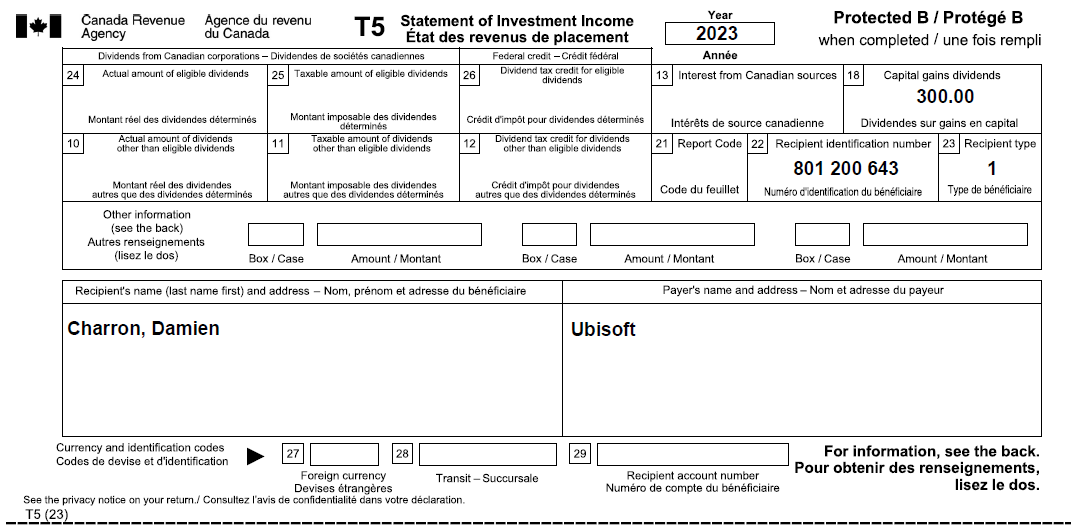
\includegraphics[width=.9\textwidth]{exercice/6-3/Q2/T5.png}
		\caption[]{Exercice 3, T5}
		\label{fig:chap6Exercice3T5}
	\end{figure}
	
	\begin{figure}
		\centering
		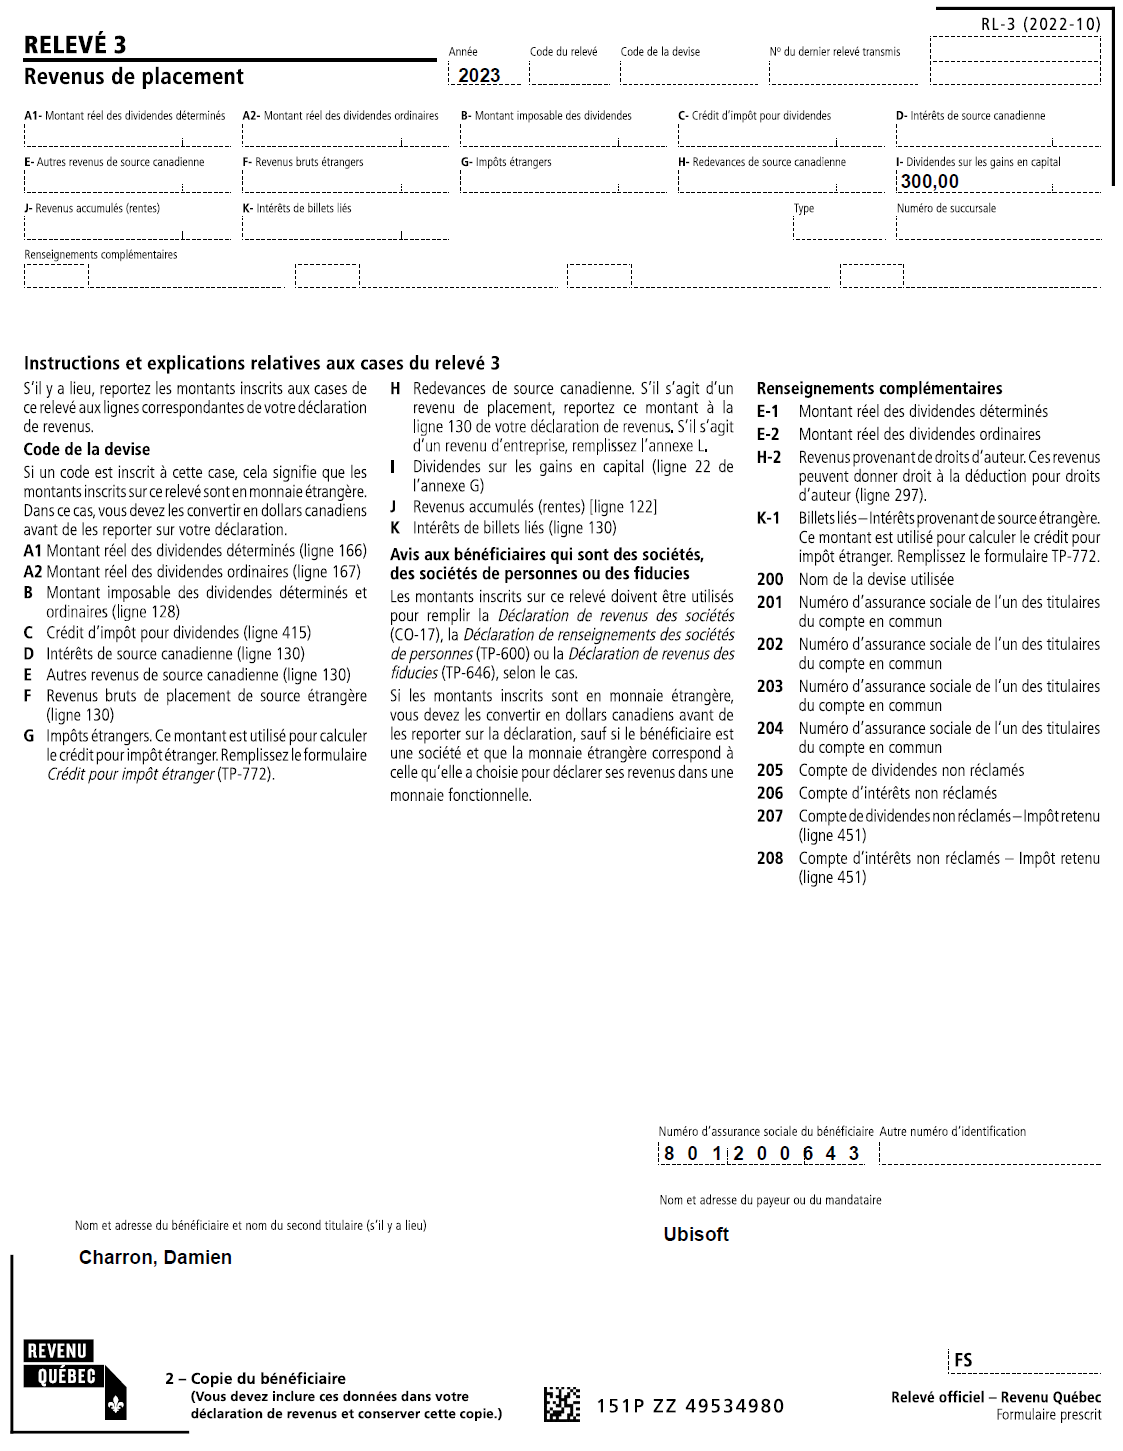
\includegraphics[width=.9\textwidth]{exercice/6-3/Q2/RL3.png}
		\caption[]{Exercice 3, RL3}
		\label{fig:chap6Exercice3RL3}
	\end{figure}
\end{question}

\setcounter{sousQuestion}{0}
\begin{sousQuestion}
	À quelle ligne des annexes 3 et G doit-il inscrire le gain en capital qu'il a réalisé? 
\end{sousQuestion}
Damien doit déclarer le gain en capital qu'il a réalisé à la ligne~17400 de l'annexe 3 et à la ligne~22 de l'annexe G.

\begin{sousQuestion}
	À quelle ligne de ses T1 et TP-1 doit-il reporter son gain en capital imposable? Quel montant doit-il y inscrire? 
\end{sousQuestion}
Damien doit déclarer 150~\$ à la ligne:
\begin{itemize}
	\item 12700 de sa T1.
	\item 139 de sa TP-1.
\end{itemize}

\begin{question}
	Michel Rousseau a ouvert un compte bancaire au nom de chacun de ses deux enfants, Jean, âgé de 15 ans, et Catherine, âgée de 19 ans. Michel est le seul qui verse de l'argent dans les deux comptes.
	
	Jean a reçu un T5 et un relevé 3 de la banque indiquant un montant de 125~\$ aux cases~13 et D. Catherine a également reçu un T5 et un relevé 3  indiquant un montant de 250\$ aux cases~13 et D.
	
	Dans les deux cas, qui doit déclarer les revenus? Expliquez votre réponse.
\end{question}
Michel doit déclarer le revenu d'intérêts de Jean, car ce dernier est un enfant mineur. Cependant, Catherine doit déclarer ses intérêts dans sa déclaration parce qu'elle est âgée de plus de 17 ans.

\begin{question}
	Hélène Cameron a déposé une partie des allocations canadienne et familiale dans le compte bancaire établi au nom de sa fille Suzanne, âgée de 10 ans. Le compte a été ouvert spécifiquement pour Suzanne.
	
	Les intérêts gagnés dans le compte sont-ils considérés comme un revenu pour la mère ou pour l'enfant? Expliquez votre réponse.
\end{question}
Les intérêts sont considérés comme le revenu de Suzanne, car ils ont été gagnés sur le dépôt des allocations canadienne et familiale dans le compte bancaire ouvert pour le bénéfice de Suzanne.

\begin{question}
	Durant l'année d'imposition, Pierre Lauzon a eu les revenus suivants:
	Revenu d'emploi\dotfill\numprint{27800}~\$
	Dividendes sur gains en capital imposables (\numprint{3200}~\$ $\times$ 50~\%)\dotfill\numprint{1600}~\$
	Dividendes déterminés imposables\dotfill\numprint{27600}~\$
	Autres revenus de placement\dotfill\numprint{34500}~\$
	
	Il a réclamé \numprint{5070}~\$ de frais financiers et de frais d'intérêts. Il se demande s'il doit cotiser au Fonds des services de santé du Québec (FSS).
\end{question}

\setcounter{sousQuestion}{0}
\begin{sousQuestion}
	Complétez l'\href{https://www.revenuquebec.ca/documents/fr/formulaires/tp/2023-12/TP-1.D.F%282023-12%29.pdf}{annexe F} de Pierre.
\end{sousQuestion}
Oui, Pierre doit cotiser 150~\$, voir l'annexe F de Pierre Lauzon figure~\ref{fig:chap6Exercice3annexeF}.

\begin{figure}
	\centering
	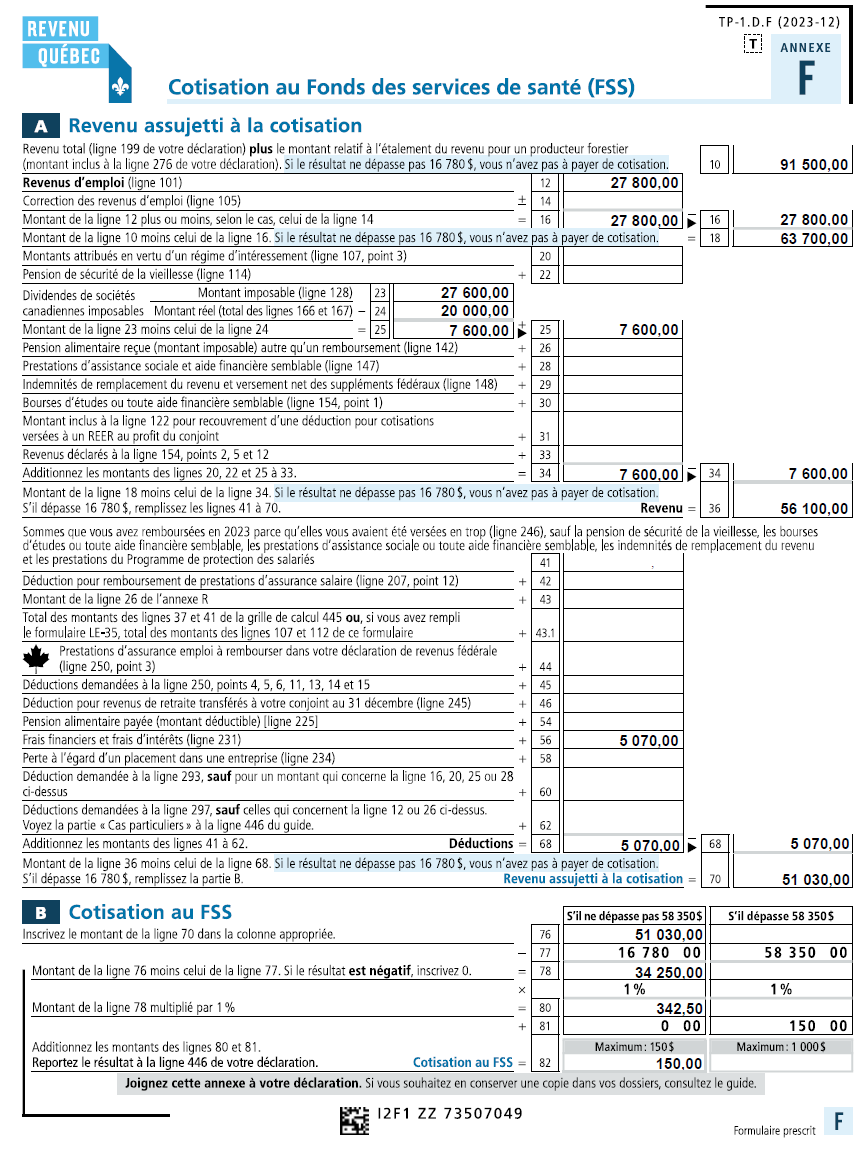
\includegraphics[width=.9\textwidth]{exercice/6-3/Q5/annexeF.png}
	\caption[]{Exercice 3, annexe F}
	\label{fig:chap6Exercice3annexeF}
\end{figure}

\begin{sousQuestion}
	À quelle ligne de la TP-1, la cotisation qui sera versée au Fonds des services de santé du Québec doit-elle être reportée?
\end{sousQuestion}
Il doit inscrire la cotisation de 150~\$ du FSS à la ligne~446 de sa TP-1.

\begin{question}
	En mars~2023, Nevena (SIN 870 201 431) a acheté un condo au deuxième étage au 28 - 742 73rd Ave, Montréal, QC, J8L 1M1 pour \numprint{300000}~\$. Au début du mois d'août, Nevena a eu un accident et est maintenant confinée en permanence dans un fauteuil roulant. Elle a vendu son condo le 25 août pour \numprint{350000}~\$ et a acheté un condo au premier étage pour y vivre à la place.
	
	La règle sur la revente précipitée de propriétés s'applique-t-elle à la vente du condo? 
\end{question}
Non, Nevena a subi un accident qui a entraîné un handicap.  C'est l'un des événements de la vie admissibles (point 5 de la ligne~17906), de sorte que l'appartement du deuxième étage n'est pas considéré comme un bien retourné, même si elle l'a possédé pendant moins d'un an.  



\section{Sommaire du chapitre}
\begin{itemize}[label=\twemoji{star}]
	\item Comment utiliser la feuille de travail fédérale pour répertorier et déclarer les dividendes, intérêts et autres frais de placement;
	\item Le traitement fiscal de la majoration et des crédits d'impôt compensatoires pour dividendes;
	\item L'intérêt est assez simple, mais il comporte souvent de nombreuses subtilités; 
	\item Comment déclarer un gain en capital simple;
	\item Déclarer la vente d'une résidence principale;
	\item Déclarer la revente précipitée de biens.
	\item Les règles d'attribution;
	\item Demander une déduction pour frais de placement;
	\item Le Fonds des services de santé.
\end{itemize}
